As long as no player stands in front of the screen, a bar is shown together with three blackboards containing the highscores. A hint invites the player to step onto the mark, which is located in front of the screen (see \autoref{fig:screenshot2}). When a player is detected, the main protagonist \ed appears. The player can now get used to the controls, without having to worry about keeping balance yet. At the same time, the player chooses the difficulty, encoded as three different alcoholic drinks: beer, wine and wodka.
\marginpar{
\begin{figure}
  \centering
  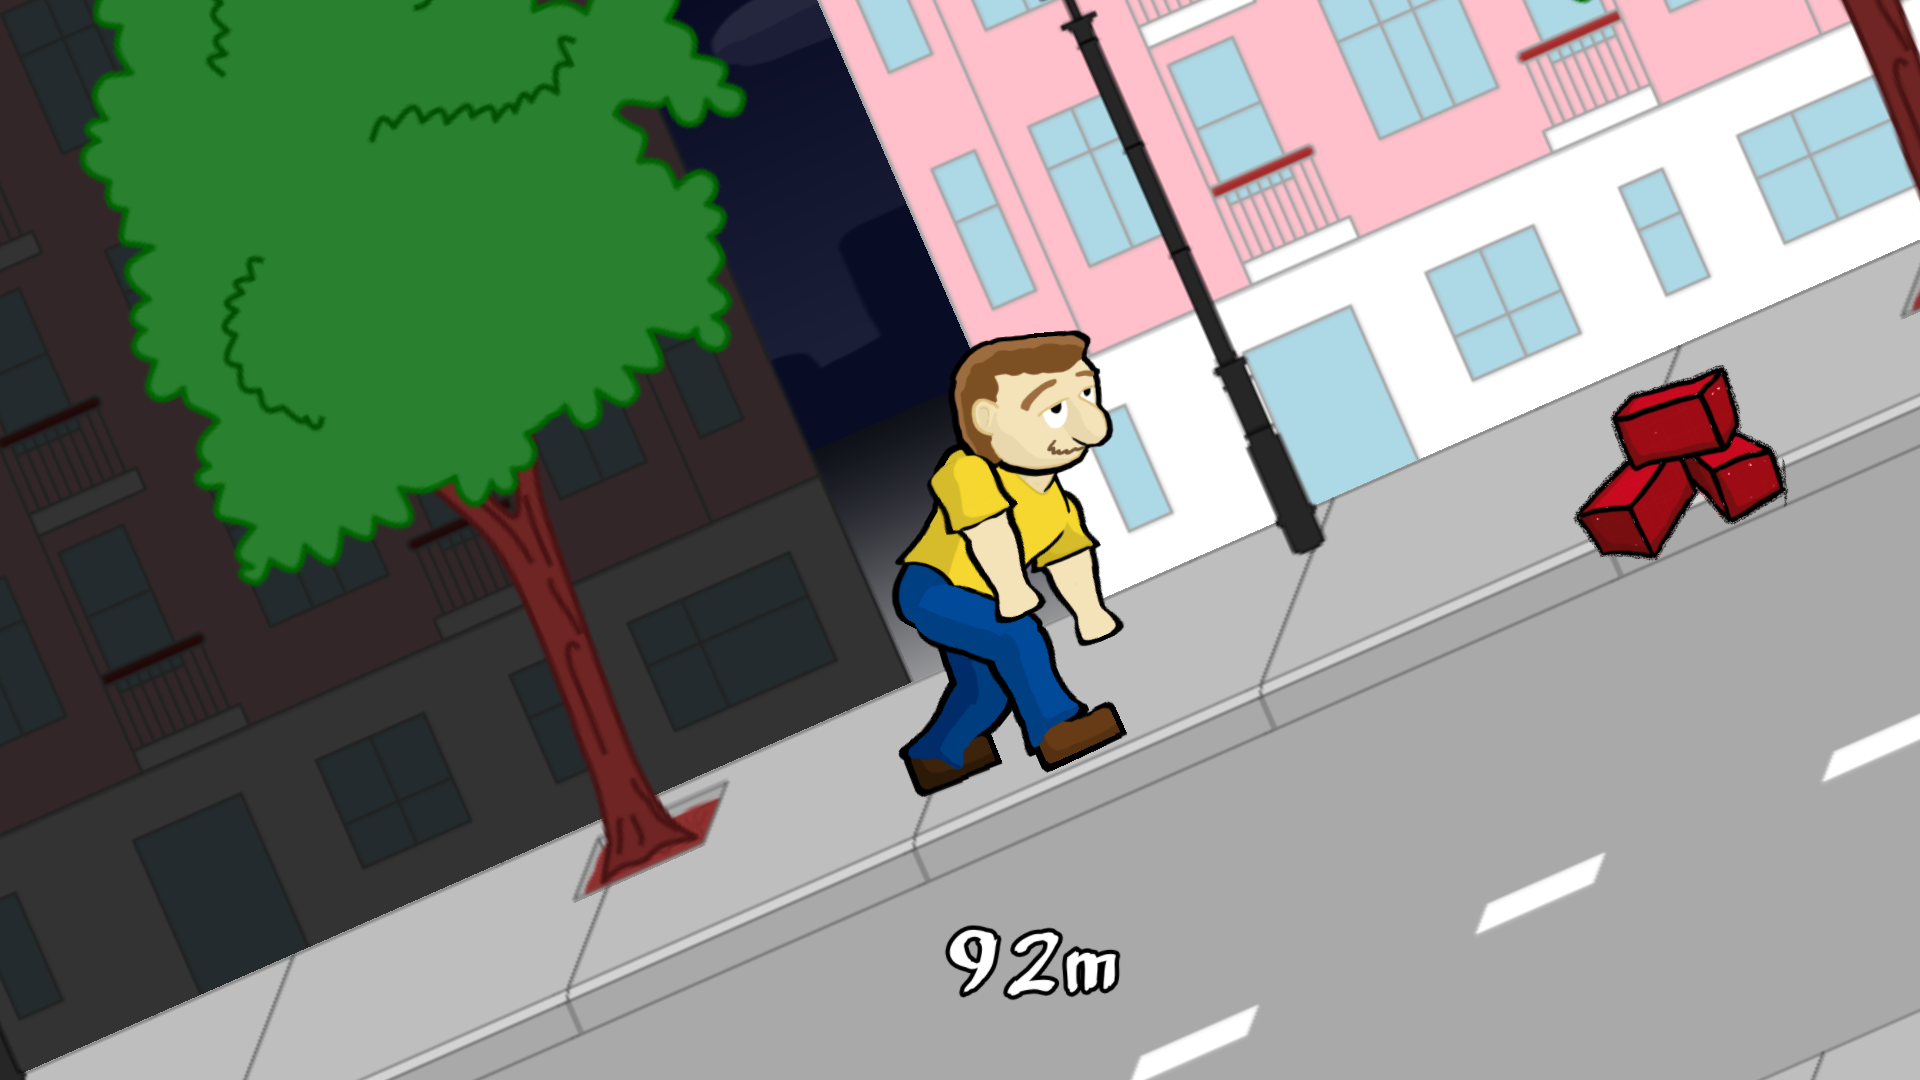
\includegraphics[width=\linewidth]{pictures/screenshot1.png}
  \caption{Insert a caption below each figure.}
  \label{fig:screenshot1}
\end{figure}
\begin{figure}
  \centering
  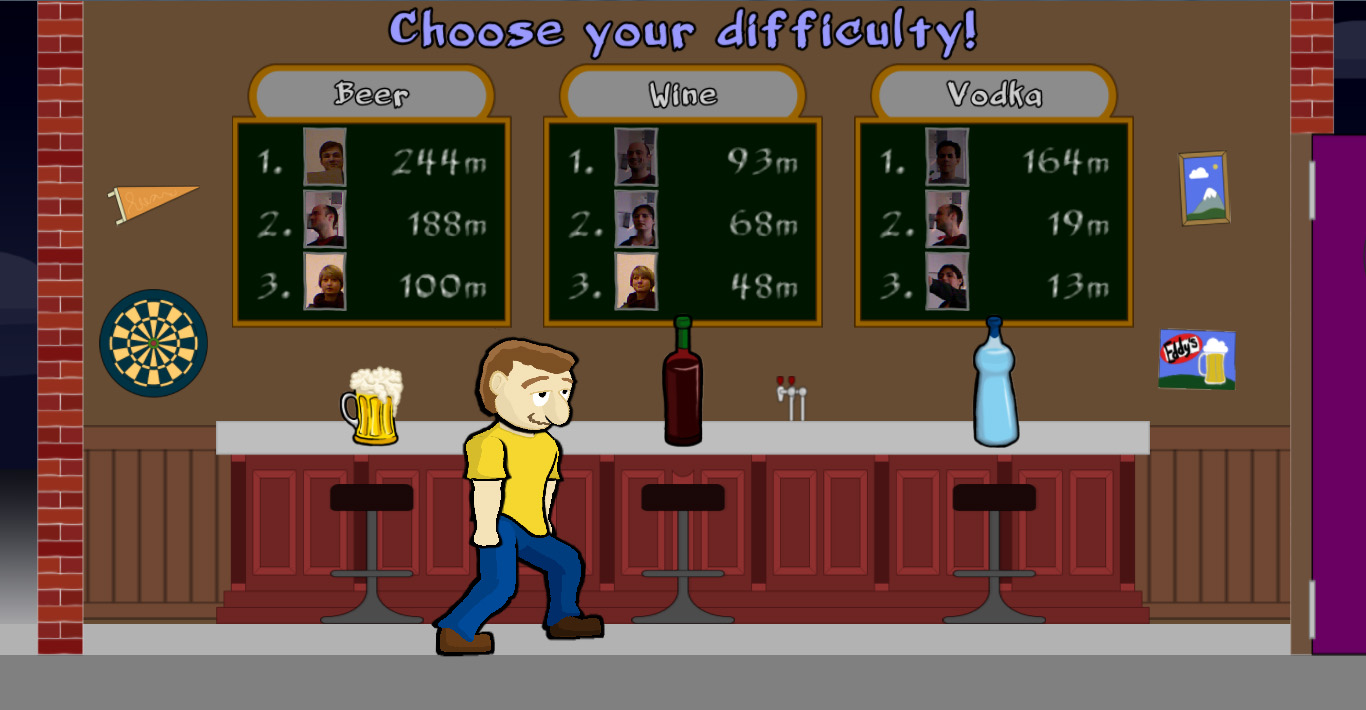
\includegraphics[width=\linewidth]{pictures/screenshot2.jpg}
  \caption{Insert a caption below each figure.}
  \label{fig:screenshot2}
\end{figure}
\begin{figure}
  \centering
  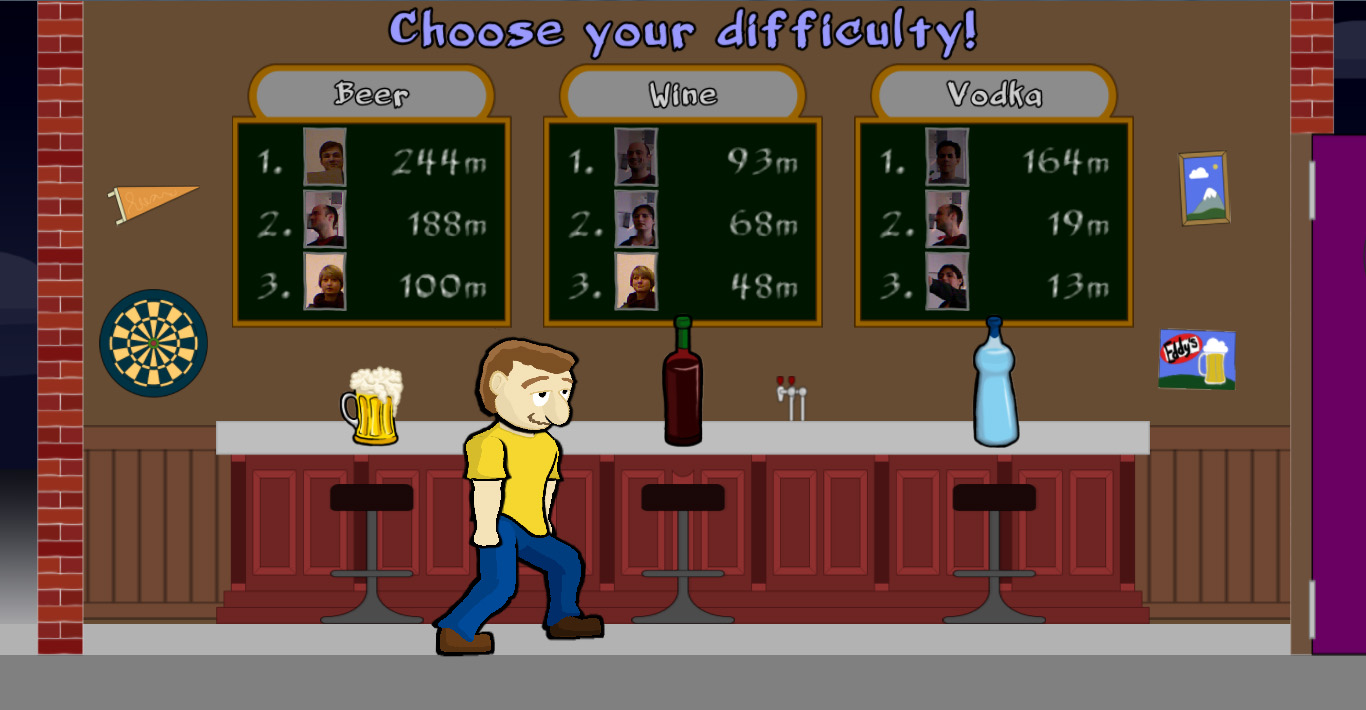
\includegraphics[width=\linewidth]{pictures/screenshot2.jpg}
  \caption{Insert a caption below each figure.}
  \label{fig:screenshot3}
\end{figure}
\begin{figure}
  \centering
  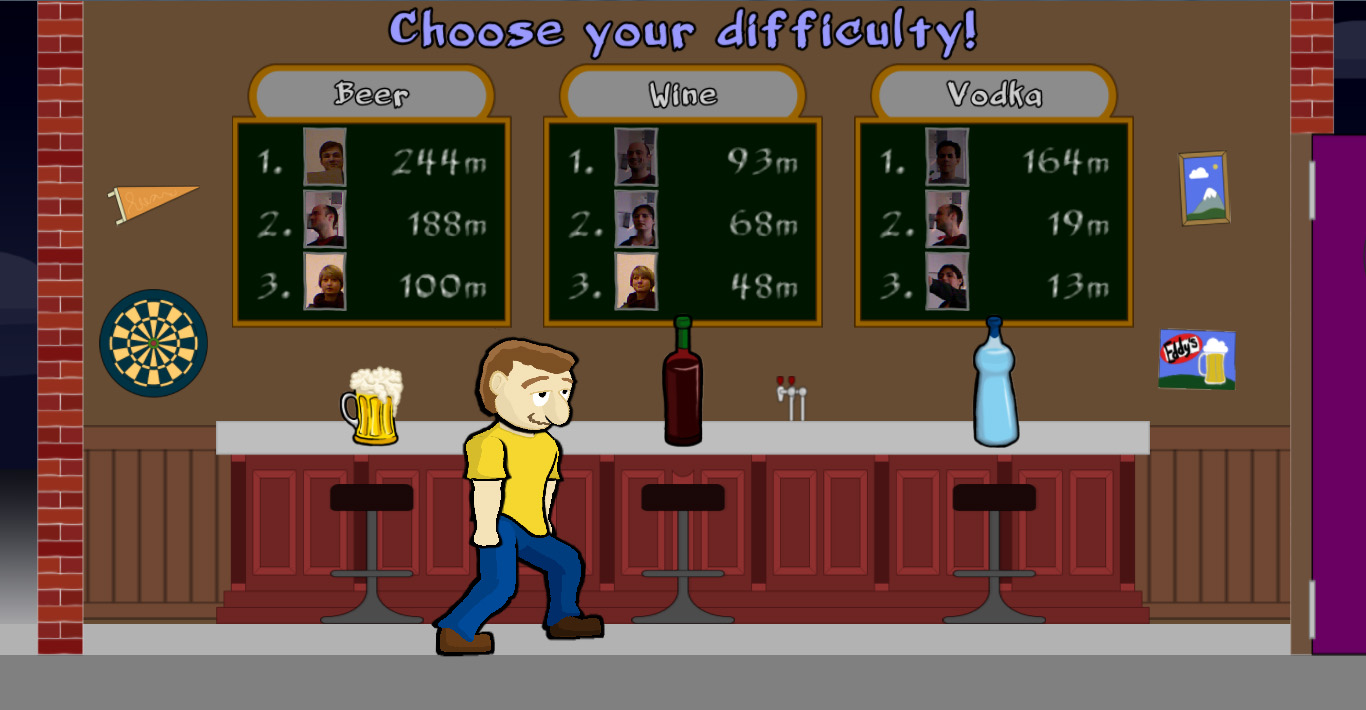
\includegraphics[width=\linewidth]{pictures/screenshot2.jpg}
  \caption{Insert a caption below each figure.}
  \label{fig:screenshot4}
\end{figure}
}
By bending him or herself, the player can move \ed\ to the respective drink. The user confirms his or her choice by performing a drinking gesture. This expressive gesture is explained by hints as proposed by Walter et al. \cite{walter2013strikeapose}\lbreak

At this point, the main game starts. The player must make \ed\ walk as far to the right as possible. \ed\ does not walk in a controlled manner, but always follows his center of mass. This resembles the typical accentuated movement of a drunken person. The player bends his or her upper body to control \eds\ upper body, which in turn shifts his center of mass. \ed\ gathers speed, the more he bends. The core mechanic is the rotating world: The upper body of \ed\ has the same orientation as that of the player with respect to the screen, but not with respect to the rotating world around \ed. Therefore, the player must compensate the world's rotation to not tumble, which happens as soon as the angle between the upper body and the floor becomes too small. Additionally, \ed\ stumbles if he goes too fast.\\
The higher the difficulty, the faster and more uncontrollably the world rotates, which makes it harder to keep balance and make \ed\ proceed to the right at the same time.\lbreak

\ed\ will eventually fall down. The game over overlay appears and the distance \ed\ walked until falling down is presented to the player as his score. If the player got a top three score, he or she can take a picture of him or herself to appear in the highscore list of the bar. The player does so by doing the drink gesture, in order that the picture captures him or her in a drinking posture. If the player does not want to take a picture, he or she has to wait for some seconds without doing anything or to leave the play area. Afterwards, the game restarts and the player gets back to the difficulty selection.\lbreak

During gameplay, the arms of \ed\ play an important role: In the difficulty selection, the arms are controllable by the players arms. However, in the main game, resembling typical cartoony postures of drunkyards, the arms are saggy, pointing straight towards the floor. Firstly, this emphasizes the loss of physical control, because the players arm movements are ignored now. Furthermore, they contribute to the players orientation, because \eds\ arms being aligned with the upper body mean a neutral posture without movement. When they are not aligned, the angle helps estimating the movement. In addition, the arms have an important feedback role: if \ed\ is getting too fast, they start to flail. If \ed\ is about to overbend, they start to swing. Players quickly understood those actions as alarming indicators.